\chapter{Literature Review}
\label{Chapter 2}

\section{History of Object Recognition \& Detection}

The field of computer vision deals with how the computers can be made to understand digital images or videos. 
The history of Computer Vision can be traced back to 1960s. Before that people had tried for alphabet recognition 
but those attempts had not led very far. L.G. Roberts, in his Ph.D thesis mentioned about the perception 
of solid objects. Using the properties of three dimensional transformations and the laws of nature, a procedure 
was developed which had been able to identify objects as well as determine their orientation and position in space \cite{chap_2_article:1}. 

In 1970s, David Marr wrote a book on visual recognition. In his book he mentioned that in order to take an 
image and to arrive at a final holistic full 3D representation of the visual world, we must go through 
several processes. The first process he calls is “Primal sketch” where edges, bars, ends and virtual lines 
are determined. Next is “two and half-D sketch” leading to “3-D sketch”  \cite{chap_2_article:2}. Another very important seminal 
group of work happened in 1970s when people began to ask the question, “how can we move beyond simple block 
world and start recognizing real objects?” Two group of scientists proposed similar ideas, one 
is called “generalized structure” and other is called “pictorial structure”. The basic idea was that 
every object is composed of simple geometric primitives \cite{chap_2_article:3}. 

In 80s, David Lowe tried to recognize razors by constructing lines and edges and mostly straight lines 
and their combination. At those times, it was very hard to solve an image recognition problem due to 
limited resources. From 1999 to 2000, statistical machine learning techniques started to gain momentum. Such 
techniques are support vector machines, boosting, graphical models etc. In 2006, FujiFilm rolled out first 
digital camera with face detection feature.

One of the very influential way of thinking in the late 90s till the first 10 years of 21st century was feature 
based recognition. An important work was done by David Lowe based on a feature called as SIFT feature. The idea 
was that to match one stop sign shown in Figure \ref{fig:2.1} with another stop sign is very difficult, because there might 
be all kinds of changes due to camera angles, occlusion, viewpoint, lighting and just the intrinsic variation of 
the object itself. Despite it is inspired to observe that there are some parts of the object that tend to remain 
unchanged. So, the task of object recognition began with identifying those features on the object and match these 
features to a similar object \cite{chap_2_article:4}.

\begin{figure}[t]
	\centering
	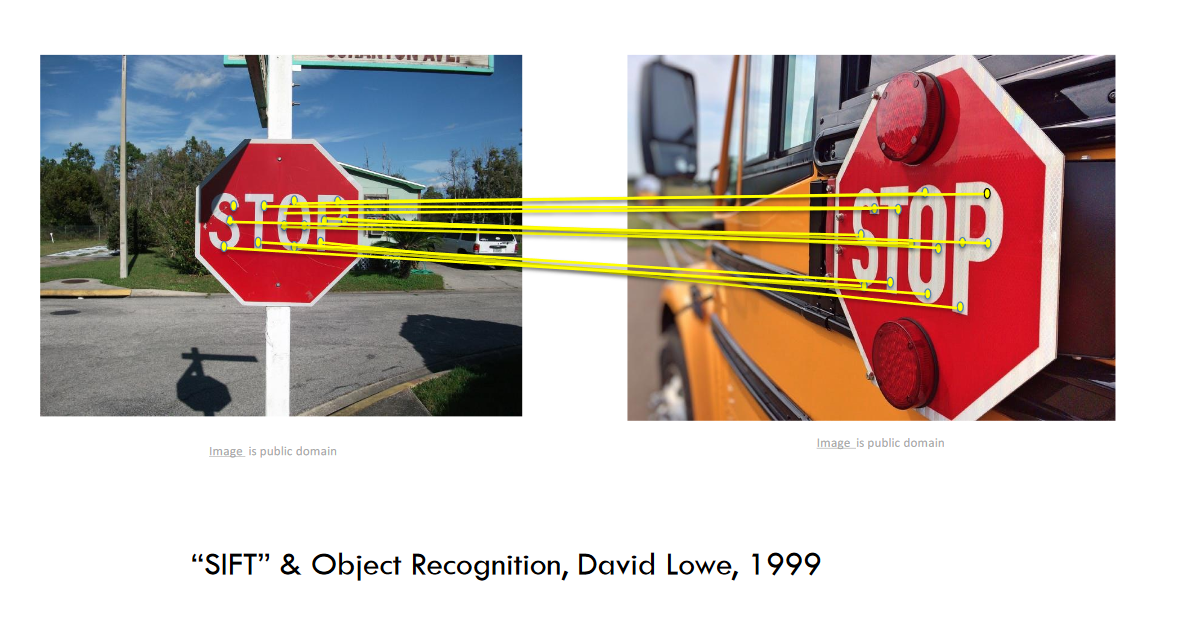
\includegraphics[width=0.80\textwidth]{CHAPTERS/Chapter-2/Images/2.1.png}
	\caption{SIFT \& Object Recognition}
	\label{fig:2.1}
\end{figure}
In 2009, the ILSVRC was 
rolled out. This data set contains 1.4 million images of different classes. In 2012, the 
error rate was dropped to almost 16 \% \cite{chap_2_article:5}. The winning algorithm was based on 
CNNs. This work was published in 2012 introducing AlexNet, which brought a tremendous change in the field of image recognition. This thesis is based on image 
classification and detection using CNNs. 

\section{Basics of an Image}
To start with, we must understand all about an image, the information of 
an image that is important to a machine. A digital image is picture 
information in digital form. It consists of pixels. The number of pixels 
in the presentation of a digital image is its spatial resolution, which 
relates to the image quality. The higher the spatial resolution, the better 
quality the image has. The resolution can be high, for instance, as high as 
1,600 $\times$ 1,200 (1,920,000 pixels = 1.92 megapixels), or as 
low as 320 $\times$ 200 (64,000 pixels = 64 kilo pixels). In notation, the number 
to the left of the multiplication symbol represents the width, and that to 
the right of the symbol represents the height. Image quality also depends on 
the numbers of bits used in encoding each pixel level \cite{chap_2_article:6,chap_2_article:7}. 

\subsection{8-Bit Gray Level Images}
If a pixel is encoded on a gray scale from 0 to 255, where 
0 corresponds to black and 255 corresponds to white. The intermediate 
numbers represent the shades of gray. For example, for a 640 $\times$ 480 bit 
image, 307.2 kilobytes are required for storage. Figure \ref{fig:2.2} shows a 
grayscale image format. The pixel value indicated 
in the box has an 8-bit value of 25. 

\begin{figure}[H]
	\centering
	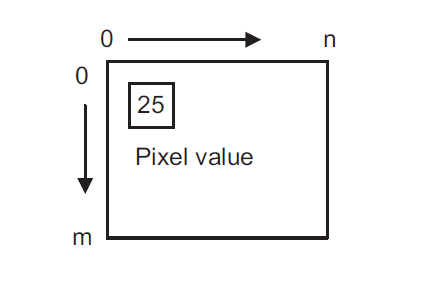
\includegraphics[scale = 0.5]{CHAPTERS/Chapter-2/Images/2.2.png}
	\caption{Grayscale Image format}
	\label{fig:2.2}
\end{figure}

\subsection{2.2	24-bit Color Images}
In a 24-bit color representation, each pixel of an image is 
encoded with Red (R), Green (G) and Blue (B) values. With each component 
encoded in 8 bits, we have a total of 24 bits for a full color RGB image. Having 
such an image, we have 2\textsuperscript{24} = 16:777216 $\times$ 10\textsuperscript{6} 
different colors. A 640 $\times$ 480 24-bit color 
image requires 921.6 kilobytes for storage. Figure 2.3 shows the format for the 24-bit 
color image where the indicated pixel has 8-bit RGB components.

\begin{figure}[H]
	\centering
	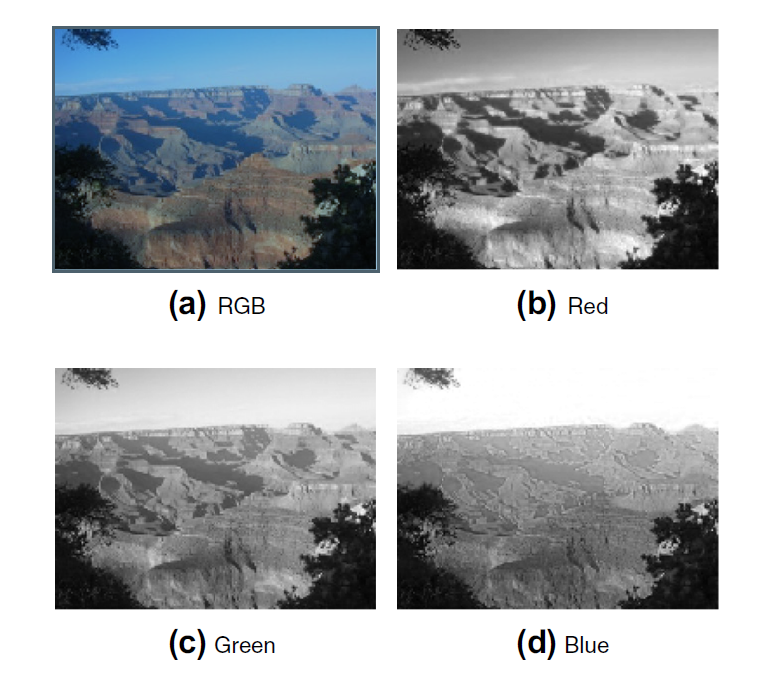
\includegraphics[width=0.80\textwidth]{CHAPTERS/Chapter-2/Images/2.3.png}
	\caption{The 24-bit color image and its RGB components}
	\label{fig:2.3}
\end{figure}

\subsection{8-Bit Color Images}
The 8-bit color image is also a popular image format. The pixel 
values are indexed from 0 to 255. Each index represents an entry of the 
color map. These images are called color indexed images. As an example, figure 2.4 shows 
a color indexed image that has a pixel value of 5, which is the index for the entry of 
the color table. At location 5 in the color table, there are three color components with 
RGB values of 66, 132 and 134 respectively. Each color component is encoded in 8 bits. There are 
only 256 different colors in the image. A 640 $\times$ 480 8-bit color image requires 307.2 kilobytes 
for data storage and 3 $\times$ 256 = 768 bytes for color map storage.

\begin{figure}[H]
	\centering
	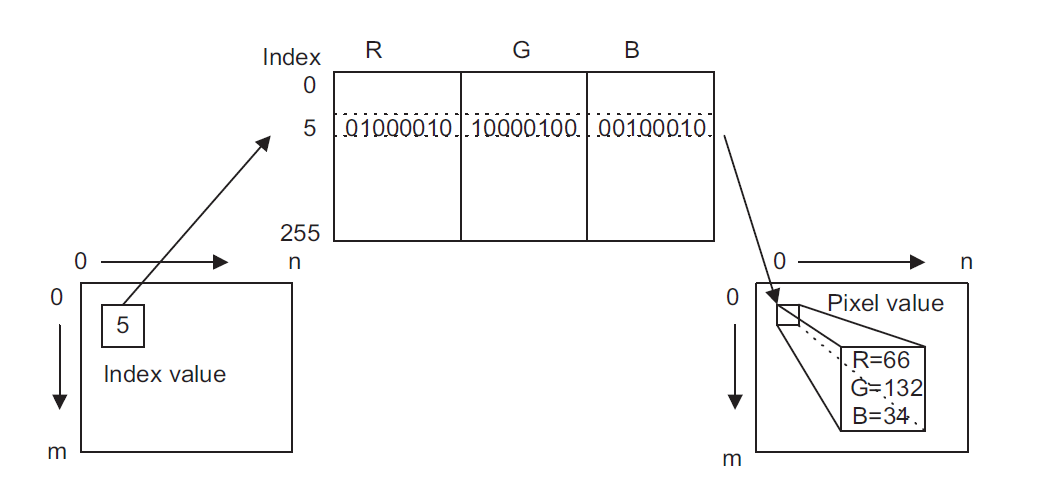
\includegraphics[width=0.80\textwidth]{CHAPTERS/Chapter-2/Images/2.4.png}
	\caption{The 8-bit color indexed image}
	\label{fig:2.4}
\end{figure}

\subsection{Intensity Images}
In section 2.1, we mentioned that a grayscale image uses a 
pixel value in the range 0-255. A 0 value represents black while 255 
represents white. In some processing environments, floating point representations 
are used. The grayscale image has an intensity value normalized from 0 to 1, where 0 is 
for black and 1 is for white. Figure 2.5 shows the format of the grayscale intensity 
image, where the indicated pixel shows the intensity value of 0.5988.

\begin{figure}[H]
	\centering
	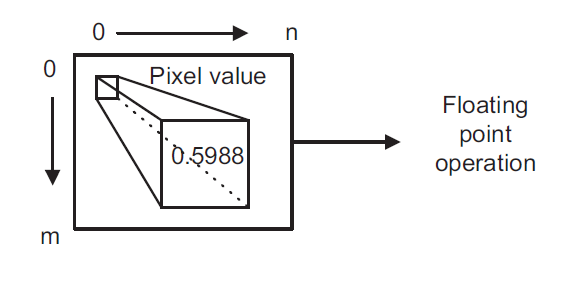
\includegraphics[scale = 0.75]{CHAPTERS/Chapter-2/Images/2.5.png}
	\caption{The grayscale intensity image format}
	\label{fig:2.5}
\end{figure}

\subsection{Red, Green, and Blue Components and Grayscale Conversion}

For processing applications, we often need to convert RGB image to grayscale. There are two popular methods, one is average method where a grayscale value is obtained by just averaging the red, green and blue pixel values. The other is luminosity method, where we use approximately 30 \% of Red, 59 \% of Green and
11\% of Blue to form a grayscale image.
\begin{equation}
	\mbox{New grayscale image} = 0.3R + 0.587G + 0.114B
\end{equation}
\section{Image Classification}
Humans can understand and depicts the information contained in an image. On the other 
hand, machines cannot identify the image and retrieve information from it on its own. To 
achieve that purpose, we make the machines learn from examples and when it has learned 
enough, it may extract information from an image from an outside world and recognize it.

There exist many algorithms for image classification. One of them is BoW 
model, which is commonly used for document classification and natural language 
processing. In addition to document classification, the BoW model can also be used for 
image classification. We extract a set of features from an image and count 
their occurrence. We have different algorithms for feature extraction. For example, in 
BoW model, SURF algorithm was used \cite{chap_2_article:8}. Other interesting image 
classification methods include texture analysis. However, a gain in performance has been 
brought by using neural networks. With the introduction of AlexNet architecture in 
2012, the error rate was dropped tremendously. Due to robustness of these 
algorithms, the CNNs are widely used for 
image classification and recognition nowadays. 

The problem of image classification can be stated as: \textit{“Given a set of 
images labeled with a single category, the machine has to predict a new set 
of images by assigning it a label and test the accuracy of the predictions”}. For 
example, in Figure \ref{fig:2.6} an image classification model takes a single image and assigns 
probabilities to 4 labels, {cat, dog, hat, mug}. The computer sees the image as a 
3D-array of numbers. The cat example image is 248 pixels wide and 400 pixels in height 
with three color channels, Red, Blue and Green, therefore, a total 
of 248 $\times$ 400 $\times$ 3  = 297,600 numbers. Each number is an integer with values 
in range 0-255. What our task is to extract out of these 
thousands of numbers, a single label, such as “cat”. 

\begin{figure}[H]
	\centering
	\captionsetup{justification=centering,margin=2cm}
	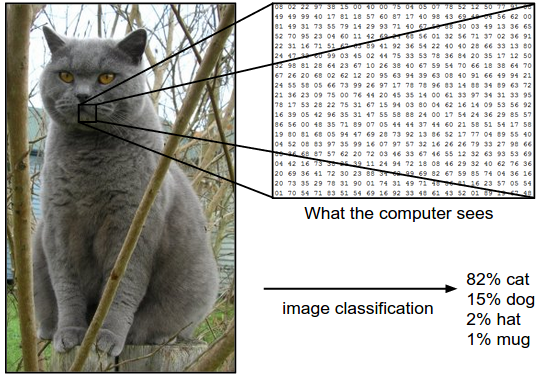
\includegraphics[width=0.80\textwidth]{CHAPTERS/Chapter-2/Images/2.6.png}
	\caption{A 3D-array of numbers from 0 to 255 of size width $\times$ height $\times$ 3. 3 represents color channels}
	\label{fig:2.6}
\end{figure}

There are a variety of challenges associated with this. There 
may exist viewpoint variation, scale variation, deformation, occlusion (a small portion 
of object is displaying), illumination conditions, background clutter and intraclass 
variations. How do we end up writing an algorithm for image classification? Researchers have 
arrived at the point that in order to solve this problem, use data-driven approach. Instead 
of writing a code to specify everyone categories of interest look like, we provide computer 
many examples of images of each class and then develop the algorithm that look at these 
examples and learn about the visual representation of each class. This approach is known 
as data-driven approach. So, the image classification pipeline can be summarized as:

\begin{itemize}
\item Input of the system is a training dataset composed 
of N images of labeled with K different classes.
\item Using this training set, we train a classifier to learn how do these classes look like.
\item After that, test this classifier on a new dataset and then compare the results with the true labels of the images.
\end{itemize}

\subsection{Convolutional Neural Networks}

CNNs are the most famous network used 
for classification problems of images. The idea behind CNNs is that a 
local understanding of an image is good enough. A practical advantage is 
that if we have fewer parameters, it will reduce the amount of data to train 
a model and improves the time of learning. A CNN has weights to look at a small 
patch of image. 

A convolution is a weighted sum of  the pixel values of an image, as 
we have a sliding window moving across the whole image. It produces another 
image of the same size. A CNN typically consists of 3 layers:

\begin{enumerate}
	\item Convolution Layer
	\item Pooling Layer
	\item Fully Connected Layer

\end{enumerate}
There are some batch normalization layers in some old CNNs 
but not used these days. (Details of CNNs are covered in chapter 3).

\subsubsection{CNN Architectures}
As mentioned before, the ImageNet project is a large visual database designed for research purposes. This 
project runs on an yearly contest named as ILSVRC, where different algorithms compete 
to classify and detect objects. Here 
we will talk about the competition top competitors \cite{chap_2_article:9}.
\begin{itemize}
	\item LeNet-5 (1998)
	\item AlexNet (2012)
	\item ZFNet (2013)
	\item GoogleNet (2014)
	\item VGGNet (2014)
	\item ResNet (2015)
\end{itemize}
\paragraph*{LeNet}

It is a pioneering 7-layer convolutional network by 
Yann LeCun et al. in 1998. It classifies digits and was applied by 
several banks to recognize handwritten numbers on cheques. The processing 
of higher resolution images we need more convolutional layers, so this 
technique is constrained by the availability of resources \cite{chap_2_article:10}.

\begin{figure}[H]
	\centering
	\captionsetup{justification=centering,margin=2cm}
	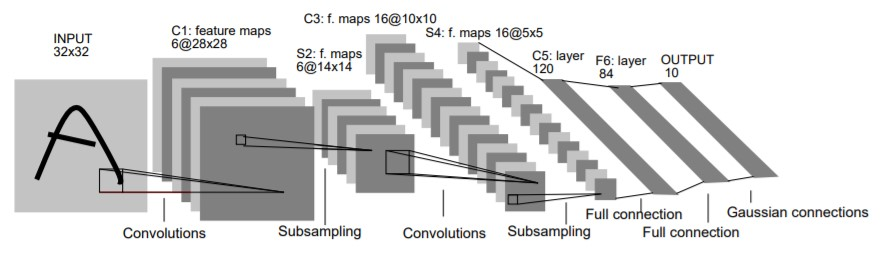
\includegraphics[scale= 0.8]{CHAPTERS/Chapter-2/Images/2.7.jpg}
	\caption{Architecture of LeNet-5, original image published in [LeCun et al., 1998]}
	\label{fig:2.7}
\end{figure}


\paragraph*{AlexNet (2012):}
In 2012, Krizhevsky et al. introduced AlexNet which 
outperformed all the prior competitors and won the challenge 
by reducing the error to 15.3 \%.  This network had a similar architecture 
like LeNet but was deeper with more filters per layer. It 
consists of 11 layers between input and output. 

 
\begin{figure}[H]
	\centering
	\captionsetup{justification=centering,margin=2cm}
	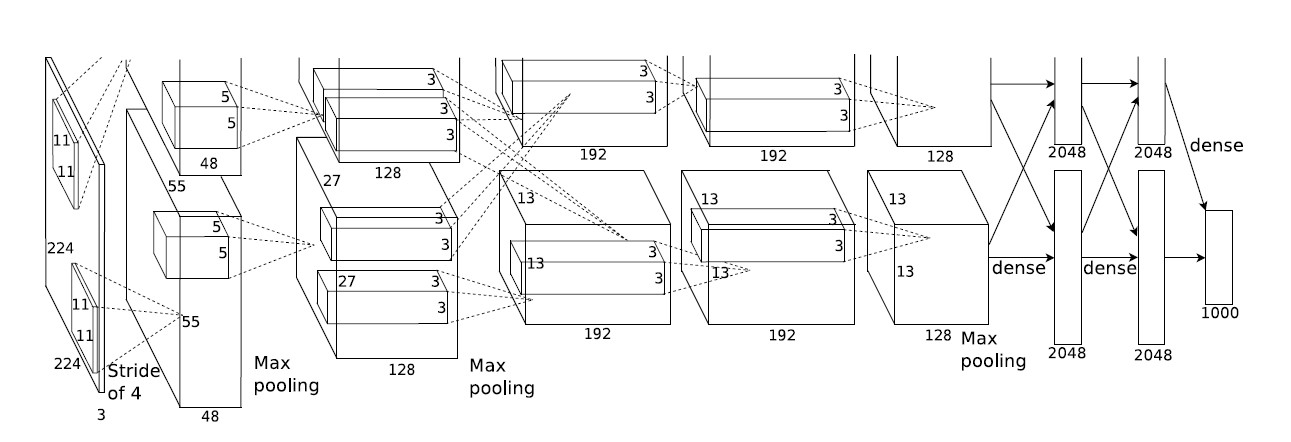
\includegraphics[scale = 0.6]{CHAPTERS/Chapter-2/Images/2.8.jpg}
	\caption{An illustration of the architecture of AlexNet CNN}
	\label{fig:2.8}
\end{figure}

\paragraph*{ZFNet (2013):}
This architecture was the winner of 2013 ILSVRC. It achieved 
an error rate of 14.8 \%. It was achieved by tweaking the 
hyperparameters of AlexNet while maintaining the same structure and 
adding deep learning elements \cite{chap_2_article:11}. The architecture 
is shown in \ref{fig:2.9}.

\begin{figure}[H]
	\centering
	\captionsetup{justification=centering,margin=2cm}
	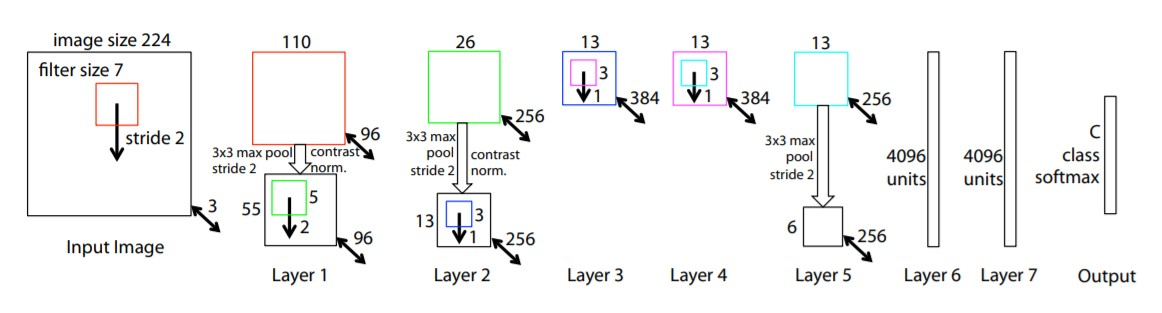
\includegraphics[scale = 0.6]{CHAPTERS/Chapter-2/Images/2.9.jpg}
	\caption{Architecture of 8 layer ZFNet Model}
	\label{fig:2.9}
\end{figure}

\paragraph*{GoogleNet (2014):}
This architecture was the winner of  ILSVRC, 2014. It achieved a top-5 
error rate of 6.67 \%. It was close to human level performance. The network 
was inspired by LeNet but implemented a new element which is dubbed an 
inception module. It used batch normalization, image distortions and RMSprop. This architecture consists of 22 layers but a 
reduced number of parameters from 60 million to 4 million \cite{chap_2_article:12}. 

\paragraph*{VGGNet (2014):}
The VGGNet was developed by Simonyan and Zisserman. It was 
runner-up in ILSVRC, 2014. It consists of 16 convolutional 
layers and popular because of its uniform architecture. A challenging thing in 
VGGNet is that it consists of 138 million parameters \cite{chap_2_article:13}.
\begin{figure}[H]
	\centering
	\captionsetup{justification=centering,margin=2cm}
	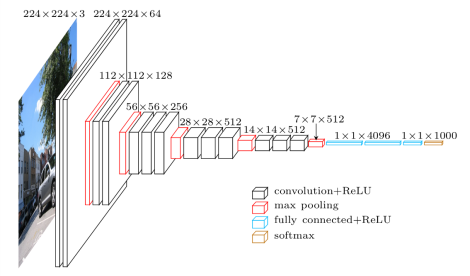
\includegraphics[scale = 0.6]{CHAPTERS/Chapter-2/Images/2.11.png}
	\caption{An illustration of the architecture of VGGNet CNN}
	\label{fig:2.10}
\end{figure}

\paragraph*{ResNet (2015):}
In 2015, Residual Neural Network (ResNet) by Kaiming He et al. was introduced. It was a novel architecture with “skip connections” and features heavy batch normalization. These connections are known as gated units. There are 152 layers but still less complex than VGGNet. It achieved a top-5 
error rate of 3.57 \% which beats human-level performance \cite{chap_2_article:14}. 

\begin{figure}[H]
	\centering
	\captionsetup{justification=centering,margin=2cm}
	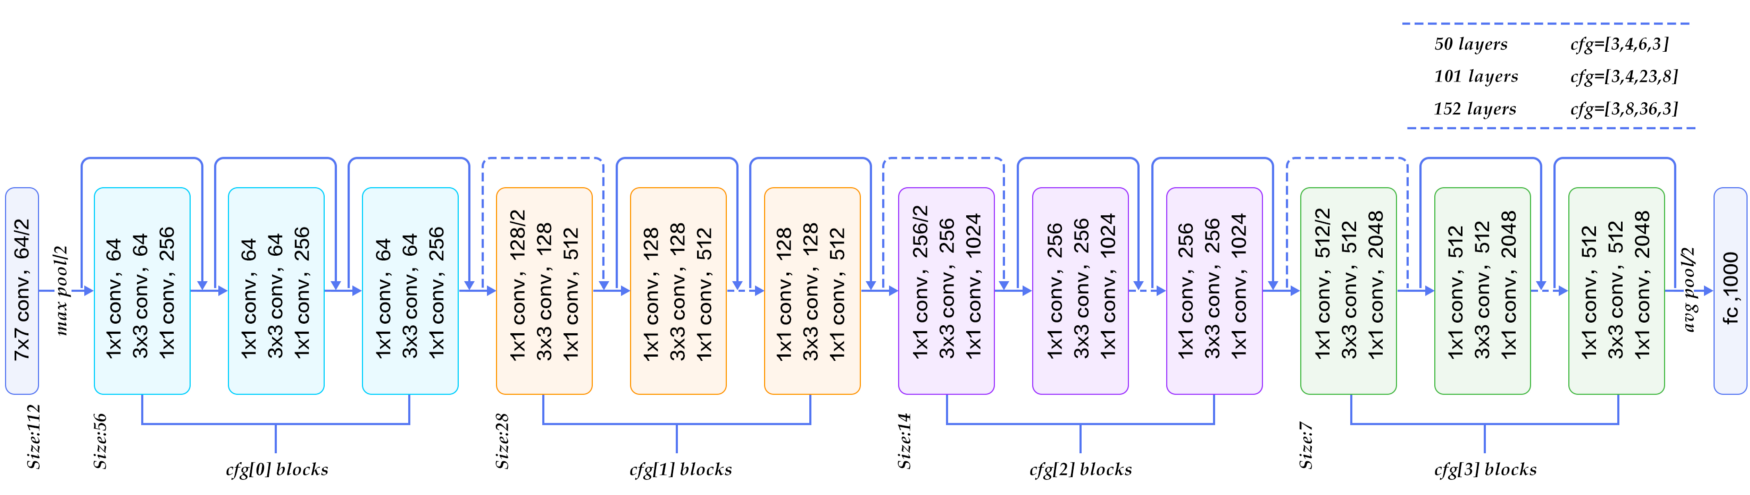
\includegraphics[width = 0.8\textwidth]{CHAPTERS/Chapter-2/Images/2.12.png}
	\caption{ResNet Architecture}
	\label{fig:2.11}
\end{figure}

AlexNet has parallel two CNN line trained on two GPUs with cross-connections, GoogleNet has 
inception modules, ResNet has residual connections.

\subsubsection*{Summary Table}
\begin{table}[H]
	\caption{Comparison of Different CNN Architectures}
	  \begin{center}
		\scalebox{.85}
		{\begin{tabular}{|l |l |l |l |l |}
		\hline
		Year & CNN & Developed by & Top-5 error rate (\%) & No. of Parameters \\ \hline
		1998  & LeNet(8) & Yann LeCun et al. &  &  60 thousand 
		\\ \hline
		2012  & AlexNet(7) & Alex Krizhevsky et al. & 60 million &
		\\ \hline
		2013   & ZFNet() &  Mathhew, Zeiler \& Rob Fergus & 9 &
		\\ \hline %
		2014 & GoogleNet(19) & Google & 6.67  & 4 million
		\\ \hline
		2014 & VGGNet(16) & Simonyan, Zisserman & 7.3 & 138 million
		\\ \hline
		2015 & ResNet(152)& Kaiming He & 3.6 & 
		\\ \hline   
		\end{tabular}}
	  \end{center}
\end{table}

